\documentclass[11pt]{article}

\usepackage[margin=1in]{geometry}
\usepackage{amsfonts,amsmath}
\usepackage{booktabs}
\usepackage{multirow}
\usepackage{graphicx}
\usepackage{xcolor}
\usepackage[colorlinks,citecolor=blue,urlcolor=blue,linkcolor=blue]{hyperref}
\usepackage[numbers,sort&compress]{natbib}
\usepackage[affil-it]{authblk}
\usepackage{lineno}

\renewcommand{\arraystretch}{1.3}
\emergencystretch=1.5em

\newcommand{\Gr}{\mathrm{Gr}}
\newcommand{\R}{\mathbb{R}}

\title{scIB Bio-Conservation Metrics Do Not Predict\\Cross-Assay Embedding Performance}

\author{Elliot Tower}
\affil{Independent Researcher \\ \texttt{elliot@elliottower.ai}}
\date{}

\begin{document}
\linenumbers
\maketitle

\begin{abstract}
Single-cell foundation models are commonly ranked using scIB
bio-conservation metrics, but whether these scores predict performance
under distribution shift is unknown. We evaluated ten scIB metrics
across trained models, conventional baselines, and null embeddings,
using cross-assay cell-type transfer as the downstream criterion.
The metrics readily distinguished trained from random embeddings and
identified the best model in 80--100\% of comparisons with clear
performance gaps. Among competitive embeddings, however, they inverted
64--86\% of pairwise rankings, yielding overall inversion rates of
46--58\%. These rankings were highly stable to Leiden resolution and
neighborhood size ($\bar{\tau} \geq 0.80$), confirming that the failure
is intrinsic rather than hyperparameter-dependent. All five
bio-conservation metrics responded non-monotonically to controlled
embedding degradation.

A pre-registered matched-assay, cross-tissue replication established
the boundary of this failure. In that setting, the scIB bio-conservation
composite positively predicted transfer performance
($\rho = 0.63$, permutation $p = 0.0014$), and the mean inversion rate
fell to 22.1\%. scIB scores retain predictive validity across
tissues within an assay platform but do not reliably rank competitive
embeddings across assay technologies. This pattern is consistent with
distance preservation in high-dimensional representations: metrics
built from distances, neighborhoods, and cluster geometry can remain
stable even when the features required for cross-assay transfer are
not preserved. Applying the same construct-validity protocol to five
geometric measures of our own eliminated four, demonstrating that the
tests are non-trivial. These results distinguish metric stability from
predictive validity and motivate a minimum standard for embedding
benchmarks: matched-dimensionality baselines, controlled degradation
tests, and direct downstream validation under the intended deployment
shift.
\end{abstract}

\noindent\textbf{Keywords:} single-cell foundation models, scIB, construct validity, embedding evaluation, cross-assay transfer


\section{Introduction}
\label{sec:intro}

Single-cell foundation model benchmarks consistently find that PCA on raw counts matches or exceeds large pretrained models across most evaluation axes \citep{wu2025scfm, vcbench2026, unifiedscfm2026, cellxgeneintegration2026}. The pattern is robust across benchmark designs. The question is whether it reflects a genuine ceiling on what training adds, or whether the evaluation metrics are insensitive to what training adds.

The field's standard evaluation suite, scIB \citep{luecken2022scib}, provides $\sim$14 metrics spanning bio-conservation (ARI, NMI, silhouette, cLISI) and batch-correction (kBET, iLISI, graph connectivity). The original paper scoped these metrics to batch-integration evaluation; recent foundation model benchmarks \citep{wu2025scfm, vcbench2026, unifiedscfm2026, cellxgeneintegration2026} adopted them for a different purpose: ranking pretrained embedding quality across models. \citet{wu2025scfm} identified the ``baselines match models'' pattern and raised the possibility that the metrics themselves might be at fault. We provide the empirical test.

We apply a three-check construct-validity protocol---null-model discrimination, cross-dimensionality robustness, sign-correctness---to the scIB suite. The metrics pass the easy check (trained $>$ random) and fail the hard one: among competitive embeddings, 64--86\% of pairwise rankings invert against ground-truth transfer F1. A pre-registered matched-assay replication establishes the boundary of this failure: scIB metrics positively predict cross-tissue transfer ($\rho = +0.63$, $p = 0.0014$) when protocol-level artifacts are removed. This pattern is consistent with distance preservation under the Johnson--Lindenstrauss lemma \citep{johnsonlindenstrauss1984}: metrics built from pairwise distances, neighbor graphs, and cluster geometry can remain stable even when the features required for cross-assay transfer are not preserved. The same confound appears in neural population geometry, where 19 geometric metrics are confounded by neuron count \citep{tower2026bracket}. To demonstrate that the validity protocol is non-trivial, we applied it to five geometric modules of our own design; it eliminated four (Supplementary~\ref{app:modules}).


\section{Results}

\subsection{scIB bio metrics pass the easy test and fail the hard one}
\label{sec:scib}

Ten scIB metrics were evaluated on six embeddings (Geneformer, scVI, scGPT, bag-of-genes PCA-512, random projection, untrained encoder) across four tissues ($n = 2{,}000$ per side). Ground-truth transfer performance is macro-averaged cell-type kNN F1 from source to target. Our claim is specific: scIB metrics lack predictive validity for cross-assay transferability, the question that current foundation model benchmarks use them to answer. A metric valid for integration evaluation may still be invalid when repurposed for model ranking.

\paragraph{Null-model discrimination.} Eight of nine testable metrics pass: trained embeddings score significantly higher than null models, with bootstrap 95\% CIs excluding zero. The largest effects are graph connectivity ($\Delta = 0.49$, CI $[0.45, 0.54]$) and NMI ($\Delta = 0.23$, CI $[0.14, 0.31]$). PCR comparison fails (CI $[-0.03, 0.46]$ includes zero). kBET returned null for all 24 conditions. scIB metrics reliably distinguish trained from random.

\paragraph{Pairwise ranking accuracy.} The harder question is \emph{which} trained model to deploy. We defined a contenders set---Geneformer, scVI, scGPT, and bag-of-genes PCA-512---and counted pairwise rank inversions against ground-truth F1 (6 pairs per tissue, 24 total).

Every bio metric inverts 46--58\% of contender comparisons, with tissue-clustered bootstrap 95\% CIs reaching or exceeding 50\% (Table~\ref{tab:scib_inversions}, Figure~\ref{fig:inversions}). Cross-tissue stability is simultaneously high (Kendall's $W > 0.80$). The metrics produce a confident, reproducible ordering that does not track downstream performance.

\begin{table}[t]
\centering
\caption{Pairwise inversion rate against ground-truth F1 on the contenders set (6 pairs $\times$ 4 tissues $= 24$ comparisons), split by F1 gap. Clear winners ($|\Delta\text{F1}| > 0.10$): the metric's ranking call matters. Near-ties ($|\Delta\text{F1}| \leq 0.10$): the correct ranking is ambiguous. Tissue-clustered bootstrap 95\% CI on the overall rate.}
\label{tab:scib_inversions}
\small
\begin{tabular}{@{}lccccc@{}}
\toprule
 & \multicolumn{2}{c}{Clear winners} & \multicolumn{2}{c}{Near-ties} & Overall \\
\cmidrule(lr){2-3}\cmidrule(lr){4-5}
Metric & inv / $n$ & rate & inv / $n$ & rate & rate [95\% CI] \\
\midrule
NMI       & 2/10 & 0.20 & 9/14  & 0.64 & 0.46 [0.33, 0.58] \\
ARI       & 0/10 & 0.00 & 11/14 & 0.79 & 0.46 [0.33, 0.58] \\
Sil-label & 2/10 & 0.20 & 11/14 & 0.79 & 0.54 [0.50, 0.63] \\
cLISI     & 2/10 & 0.20 & 12/14 & 0.86 & 0.58 [0.42, 0.75] \\
Iso-label & 2/10 & 0.20 & 12/14 & 0.86 & 0.58 [0.50, 0.67] \\
\bottomrule
\end{tabular}
\end{table}

\begin{figure}[tb]
\centering
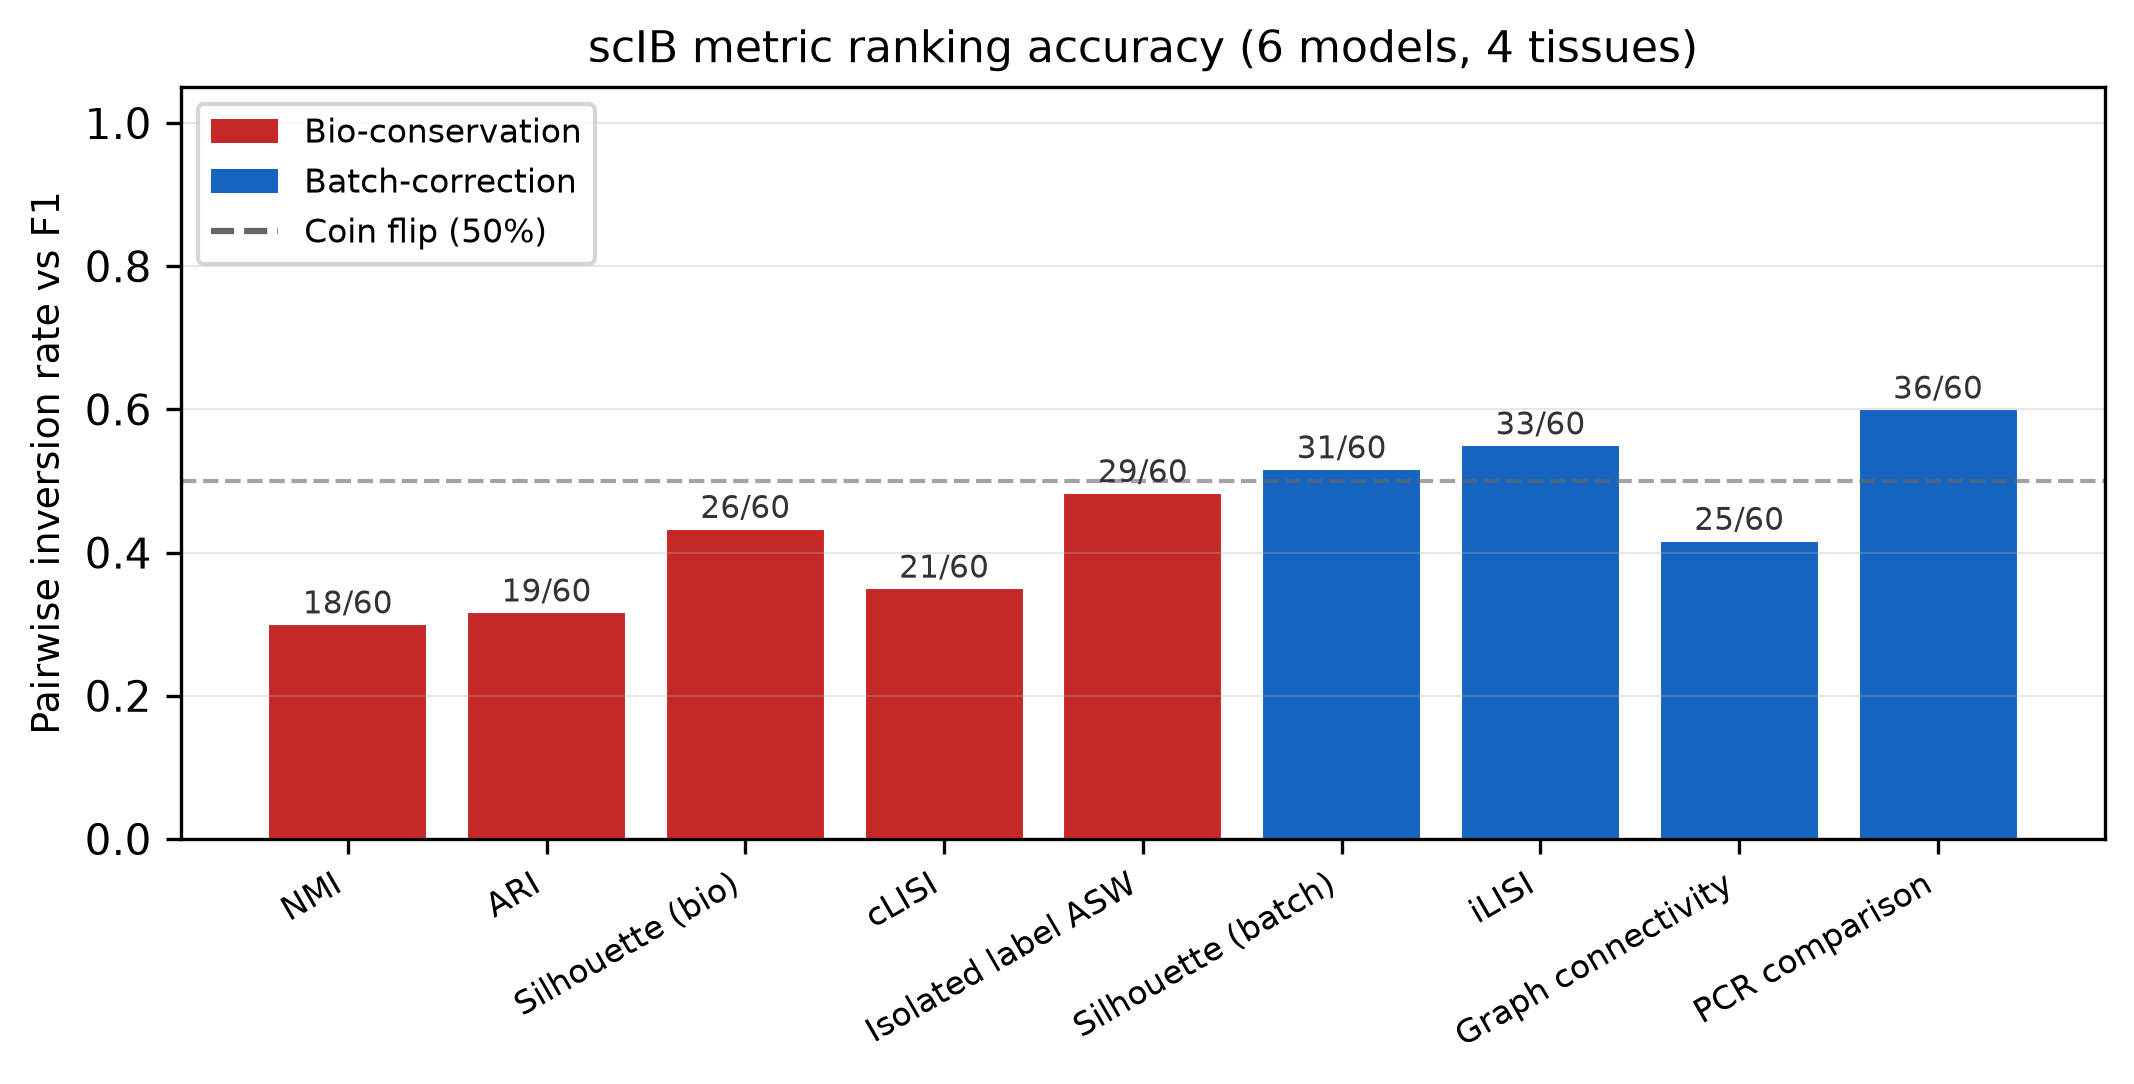
\includegraphics[width=0.7\textwidth]{figures/inversion_rates.pdf}
\caption{Pairwise inversion rates against ground-truth transfer F1 on the contenders set (4 embeddings, 6 pairs $\times$ 4 tissues $= 24$ comparisons). Bio-conservation metrics (red) invert 46--58\% of comparisons; batch-correction metrics (blue) range from 46\% to 67\%. Dashed line: coin flip. kBET excluded (all null).}
\label{fig:inversions}
\end{figure}

\paragraph{Three tiers of predictive accuracy.} The F1-gap split reveals a graded pattern (Table~\ref{tab:scib_inversions}). On clear-gap comparisons ($|\Delta\text{F1}| > 0.10$), scIB metrics correctly identify the best model (Geneformer) at 80--100\% accuracy. Among the remaining models (scVI, scGPT, BoG-PCA), all 14 near-tie comparisons hit 64--86\% inversion rates---worse than chance. In kidney, scVI and scGPT outscore BoG-PCA on every bio metric while BoG-PCA achieves 0.15--0.20 higher transfer F1. The metrics confidently prefer trained models over a baseline that actually transfers better.

scIB bio metrics reward cluster compactness of known cell types, a property that trained-versus-random separates easily. Ranking competitive embeddings by transfer quality requires sensitivity to cross-assay alignment, a property the suite was not designed to measure.

\paragraph{Suite redundancy.} The 10-metric suite has approximately 3--4 independent signals. NMI and ARI are near-identical ($\rho = 0.91$); cLISI is rank-redundant with NMI ($\rho = 0.86$) despite having almost no dynamic range (all scores $> 0.90$). The effective bio-conservation signal is carried by NMI-or-ARI plus silhouette-label; the effective batch signal is graph connectivity alone (iLISI near-zero everywhere, PCR comparison undefined on most conditions). Reporting a single ``scIB overall score'' collapses a genuine bio--batch tradeoff into a single scalar that double-counts the NMI--ARI axis.


\subsection{Cross-tissue replication localizes the failure}
\label{sec:crosstissue}

The same four contenders were evaluated on six cross-tissue pairs at matched assay (10x 3$'$ v3 $\rightarrow$ 10x 3$'$ v3, different tissues; $n = 24$ conditions), with logistic-regression cell-type F1 as ground truth.

The grand mean bio-metric inversion rate against cross-tissue F1 is 22.1\% [95\% CI: 13.1\%, 34.9\%], well below the 46--58\% observed on cross-assay transfer. The scIB bio composite positively predicts cross-tissue F1 ($\rho = +0.63$, permutation $p = 0.0014$, 95\% CI $[0.43, 0.83]$), opposite to the cross-assay result ($\rho = -0.76$). Clear-gap inversions are rare (7.3\%, $n = 110$). A seed-stability check confirms robustness: grand mean inversion rate range $[0.18, 0.22]$ across three seeds, $\rho$ range $[0.63, 0.76]$.

The failure is specific to the cross-assay setting. Matched-assay transfer removes the protocol-artifact axis (capture efficiency, UMI distributions, gene detection sensitivity), and the metrics recover predictive validity. scIB bio rankings can be trusted across tissues at matched assay but require downstream-probe validation when comparing across assays.


\subsection{Confirmatory tests}
\label{sec:confirmatory}

\paragraph{Hyperparameter sensitivity.} Kendall's $\tau$ between embedding rankings at extreme hyperparameter settings (Leiden $r = 0.5$ vs.\ $2.0$; kNN $k = 15$ vs.\ $90$) is uniformly high (Table~\ref{tab:hyperparam}). NMI rankings are perfectly preserved in three of four tissues ($\tau = 1.0$; mean extreme $\tau = 0.93$). ARI shows the largest variation ($\tau = 0.47$ in brain) but still exceeds the predicted ceiling of $0.6$. Only 1 of 16 metric $\times$ tissue combinations produced a winner change. Pre-registered predictions substantially underestimated stability---all six predictions were wrong in the same direction.

\begin{table}[t]
\centering
\caption{Hyperparameter sensitivity (confirmatory). Kendall's $\tau$ between embedding rankings at extreme hyperparameter settings (Leiden $r = 0.5$ vs $2.0$; kNN $k = 15$ vs $90$), across four tissues. All predictions underestimated stability. kBET returned null for all conditions; iLISI near-zero for most, making $\tau$ undefined. 0/6 predictions in range.}
\label{tab:hyperparam}
\small
\begin{tabular}{@{}lcccccc@{}}
\toprule
 & \multicolumn{4}{c}{Extreme-pair $\tau$} & Mean & Predicted \\
\cmidrule(lr){2-5}
Metric & Lung & Liver & Kidney & Brain & $\bar{\tau}$ & range \\
\midrule
NMI & 1.00 & 1.00 & 1.00 & 0.73 & 0.93 & 0.5--0.7 \\
ARI & 0.87 & 0.87 & 1.00 & 0.47 & 0.80 & 0.4--0.6 \\
cLISI & 1.00 & 0.97 & 0.87 & 1.00 & 0.96 & 0.3--0.6 \\
Graph conn. & 0.87 & 1.00 & 0.87 & 1.00 & 0.93 & 0.3--0.6 \\
iLISI & 0.58 & 0.67 & NaN & NaN & NaN & 0.2--0.5 \\
kBET & \multicolumn{4}{c}{all null} & N/A & 0.1--0.4 \\
\bottomrule
\end{tabular}
\end{table}

The inversions are not artifacts of hyperparameter choice: the metrics produce the same rankings regardless of resolution or neighborhood size.

\paragraph{Noise dose-response.} We apply additive Gaussian noise at $\sigma \in \{0.01, \ldots, 2.0\} \times \text{embedding\_std}$ across 24 conditions. A metric fails if non-monotonic in more than 1 of 24 conditions (Table~\ref{tab:noise}).

The results split along the bio/batch axis (Table~\ref{tab:noise}, Figure~\ref{fig:noise}). Every bio-conservation metric fails: NMI (17/24 non-monotonic), ARI (22/24), cLISI (11/24), isolated-label ASW (9/24), silhouette-label (3/24). Both batch-correction metrics with computable values pass: silhouette-batch and pcr-comparison increase monotonically in 23/24 conditions. Graph connectivity fails (22/24). kBET returned null for all 168 evaluations.

\begin{table}[t]
\centering
\caption{Noise dose-response (confirmatory). Non-monotonicity count across 24 conditions (4 tissues $\times$ 6 embeddings) at 7 noise levels ($\sigma \in \{0.01, \ldots, 2.0\} \times \text{embedding\_std}$). A metric FAILS if non-monotonic in $>1$ condition. All bio-conservation metrics fail; both computable batch metrics pass. kBET returned null for all 168 evaluations.}
\label{tab:noise}
\small
\begin{tabular}{@{}lcccl@{}}
\toprule
Metric & Non-mono & Predicted & Actual & Direction \\
\midrule
NMI & 17/24 & FAIL & FAIL & --- \\
ARI & 22/24 & FAIL & FAIL & --- \\
Silhouette label & 3/24 & PASS & FAIL & --- \\
cLISI & 11/24 & PASS & FAIL & --- \\
Isolated label ASW & 9/24 & PASS & FAIL & --- \\
\midrule
Silhouette batch & 1/24 & PASS & PASS & $\uparrow$ (23/23 non-decreasing) \\
iLISI & 2/24 & PASS & FAIL & --- \\
kBET & 0/0 & FAIL & PASS$^*$ & all null \\
Graph connectivity & 22/24 & PASS & FAIL & --- \\
PCR comparison & 1/24 & PASS & PASS & $\uparrow$ (23/23 non-decreasing) \\
\bottomrule
\multicolumn{5}{@{}l@{}}{\footnotesize $^*$kBET returned null for all 168 evaluations; PASS is vacuous.}
\end{tabular}
\end{table}

\begin{figure}[tb]
\centering
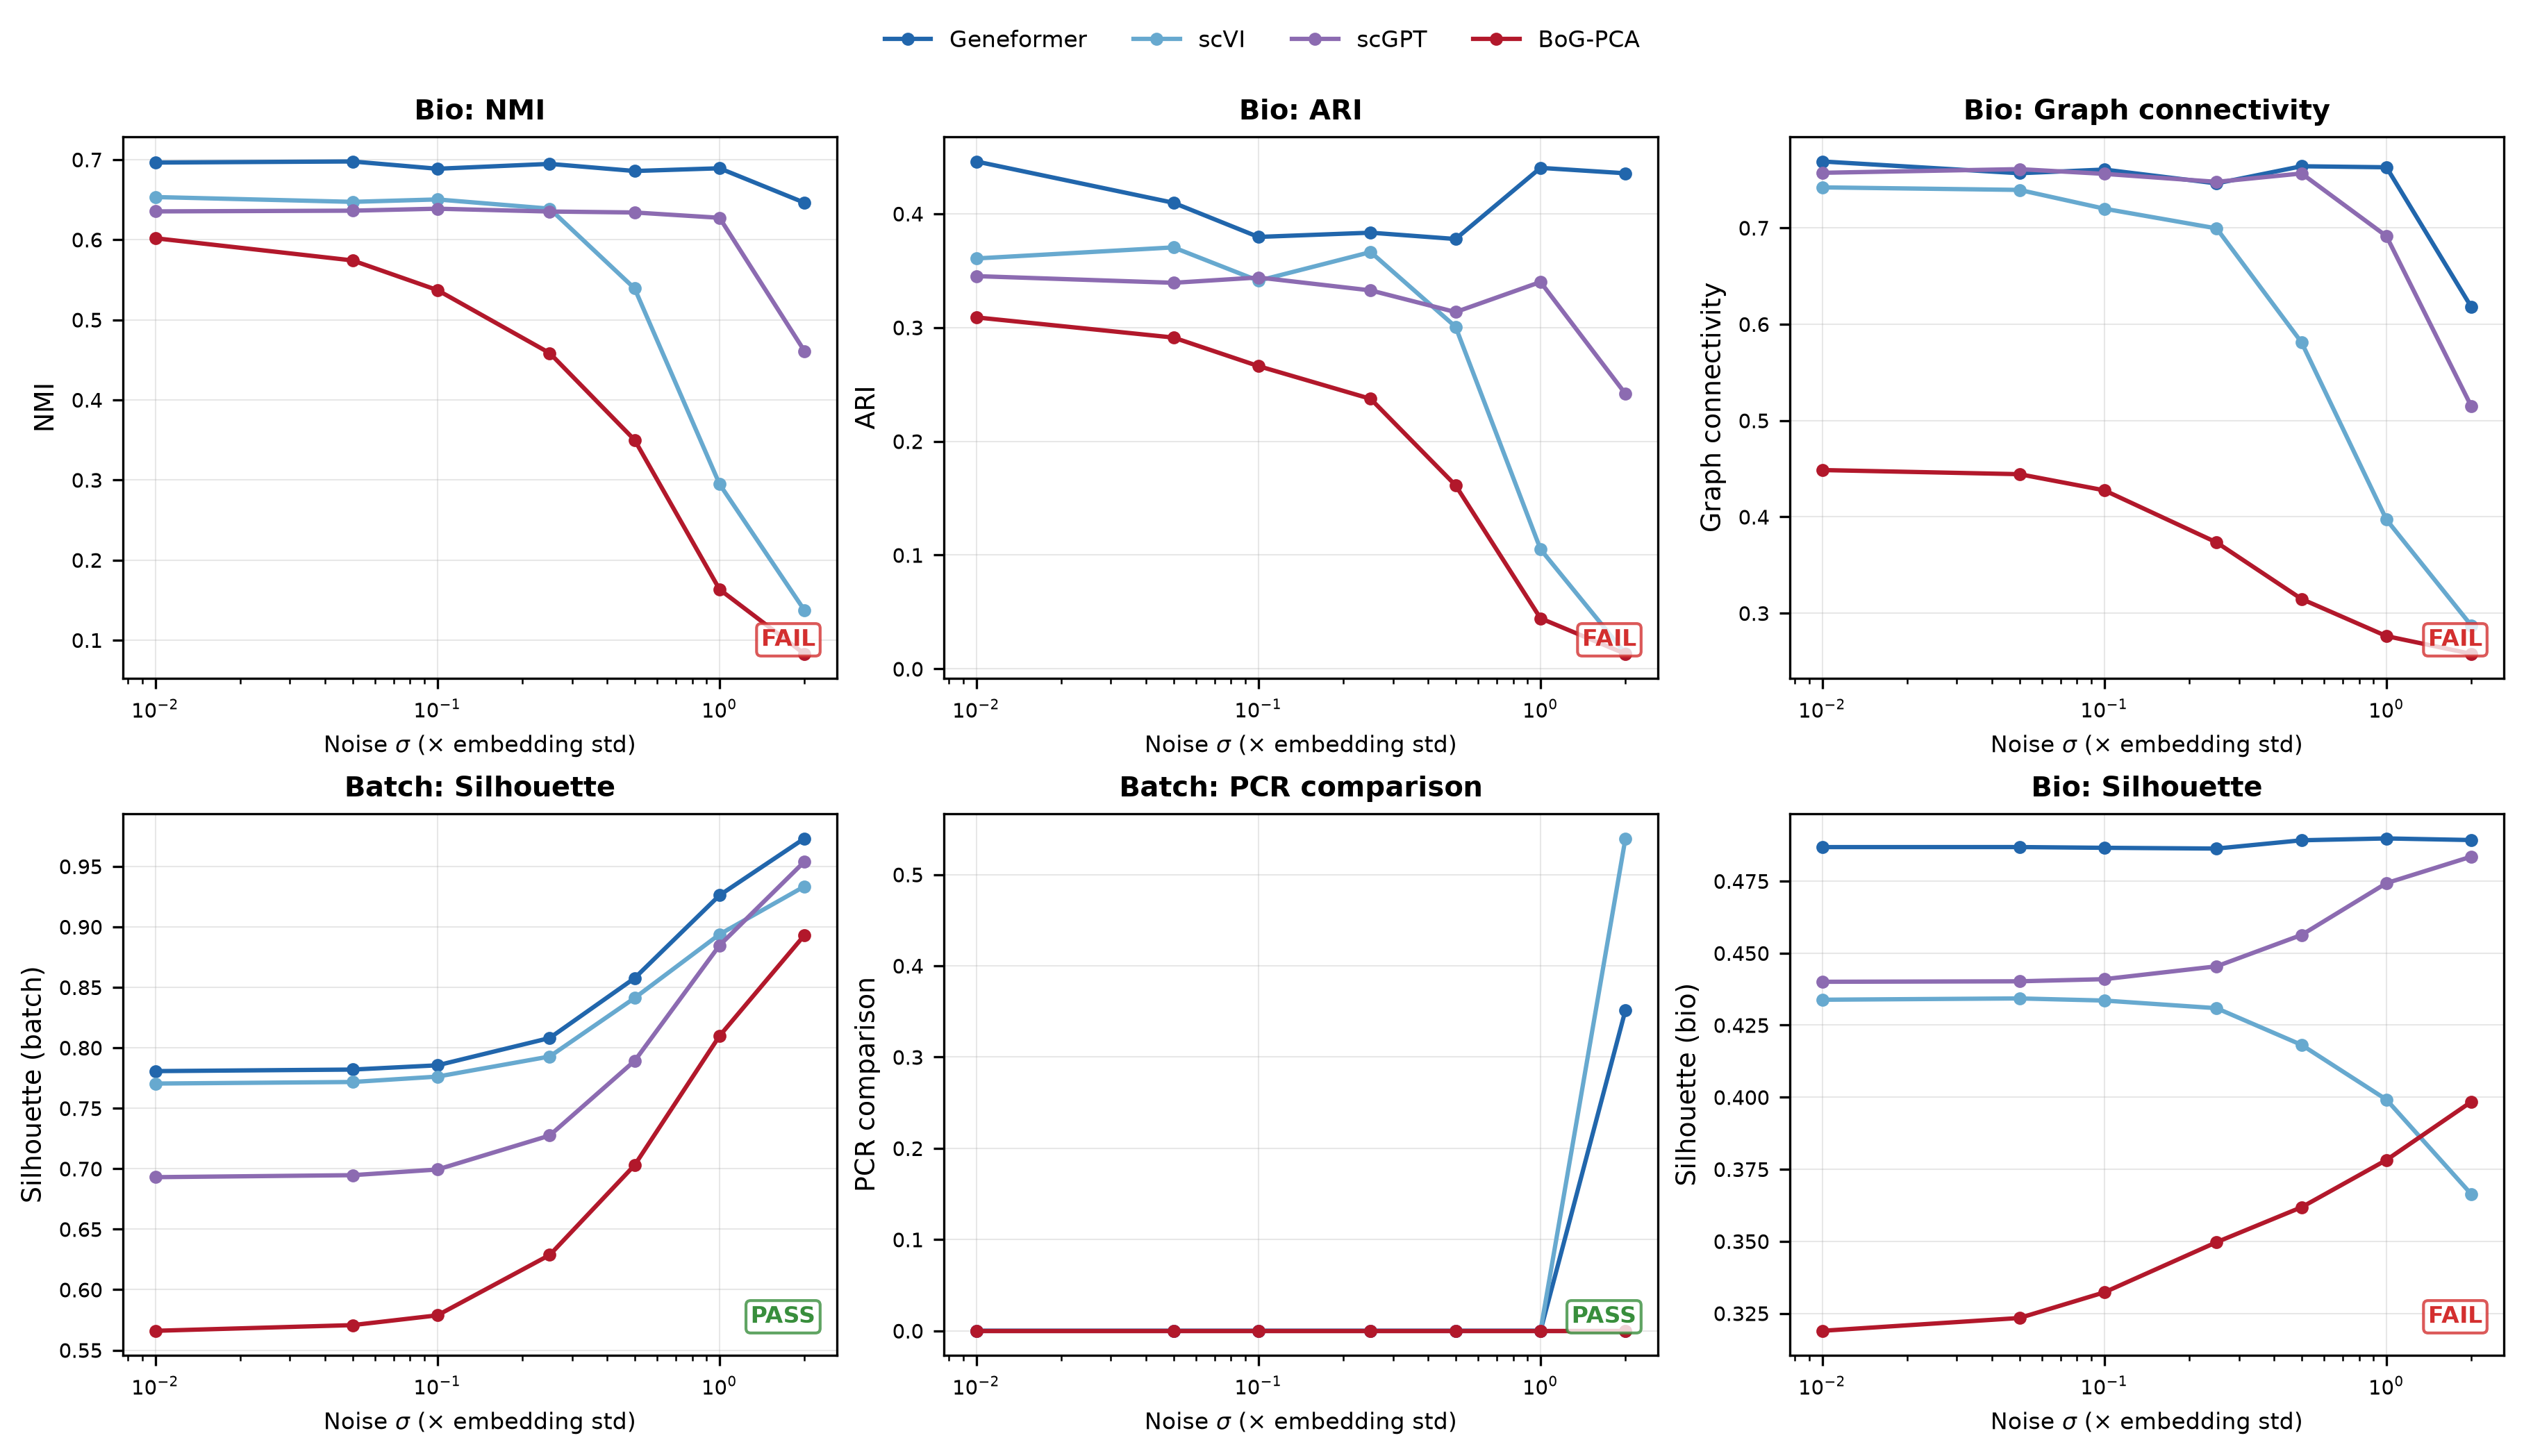
\includegraphics[width=\textwidth]{figures/noise_dose_response.pdf}
\caption{Noise dose-response for six scIB metrics on lung tissue (4 trained embeddings). \textbf{Top}: bio-conservation metrics respond non-monotonically---values increase at intermediate $\sigma$ before collapsing. \textbf{Bottom left}: silhouette-batch increases monotonically (noise destroys batch structure; mechanical PASS). \textbf{Bottom center}: PCR comparison is zero except at $\sigma = 2.0$ (mechanical PASS). $\sigma$ scaled by embedding standard deviation. Full data: Appendix~\ref{app:noise}.}
\label{fig:noise}
\end{figure}

The two tests reveal complementary failure modes. Rankings are stable (inversions are intrinsic); values are non-monotonic under degradation. Graph connectivity illustrates both simultaneously: near-perfect ranking stability ($\bar{\tau} = 0.93$) coexisting with pervasive non-monotonicity (22/24 conditions). The two surviving metrics (silhouette-batch, pcr-comparison) pass for a mechanical reason: noise destroys batch structure, so batch-mixing scores improve monotonically regardless of embedding quality. No scIB metric survives both tests as a reliable indicator of bio-conservation quality.


\subsection{The kidney inversion}
\label{sec:kidney}

The most concrete consequence: in kidney, every scIB bio metric ranks scVI and scGPT above bag-of-genes PCA-512. Ground-truth transfer F1 reverses this---BoG-PCA achieves 0.15--0.20 higher cross-assay F1. A practitioner following scIB rankings would deploy the worse embedding.

Applying the same validity protocol to five geometric modules of our own design eliminated four (Supplementary~\ref{app:modules}), demonstrating that the checks produce negative results even for metrics designed by the protocol's authors.


\section{Methods}

\subsection{Data}

All embeddings are accessed via the CellxGene Census API (v2023-12-15) \citep{abdulla2025cellxgene}. Cross-assay pairs compare 10x Chromium 3' v3 (source) against Smart-seq2 (target) within the same tissue, with zero donor overlap enforced by metadata filtering. Five tissues were initially planned; heart was excluded because Census returned zero Smart-seq2 target cells after metadata filtering, leaving four: lung (191K source, 42K target available), liver (191K source, 42K target), kidney (121K source, 4.3K target), and brain (available counts vary by model). All evaluations subsample $n = 2{,}000$ cells per side. Five embedding methods: Geneformer ($d = 512$) \citep{theodoris2023geneformer}, scGPT ($d = 512$) \citep{cui2024scgpt}, scVI ($d = 50$) \citep{lopez2018scvi}, UCE ($d = 1{,}280$) \citep{rosen2026uce}, and bag-of-genes PCA-512 ($d = 512$; $\log(1 + x)$ without total-count normalization, PCA with fixed seed; following \citealp{cole2026morpheus}). Two null baselines: random Gaussian projection ($R \in \mathbb{R}^{512 \times G}$, $R_{ij} \sim \mathcal{N}(0, 1/\sqrt{512})$) and an untrained two-layer MLP encoder (random weights, $d = 512$).

\paragraph{Handling scVI's fixed dimension.} scVI produces $d = 50$ embeddings by default. We include scVI in all analyses where dimension is not a controlled variable but exclude it from matched-dimensionality comparisons.

\subsection{Geometric modules}

Five geometric modules for evaluating embedding transportability---subspace alignment (M1), domain separability (M2), direction stability (M3), participation ratio (M4), and graph curvature (M6)---are pre-registered and applied alongside the scIB audit. Definitions and per-module results are in Supplementary~\ref{app:modules}.

\subsection{Pre-registration}

Scorer source code, hyperparameters, dataset specifications, and hypothesis thresholds were frozen via SHA-256 hashing before data access. SHA-256 hashes and the full deviation log are in the online repository.

\subsection{Statistical methods}

All correlations are Spearman rank with $10{,}000$-resample bootstrap 95\% CIs and $10{,}000$-permutation exact $p$-values. Partial Spearman correlations control for embedding dimension via rank residuals; within the 512d panel ($n = 12$), the partial $\rho$ for M1 controlling for tissue is $-0.71$ ($p = 0.009$). All transfer correlations rest on $n = 12$--$20$ conditions; we apply the power caveat symmetrically to anti-predictive and positive-but-non-significant results. Applying Benjamini--Hochberg correction at $\alpha = 0.05$ to the five overall-rate CIs does not change any conclusion.


\section{Discussion}
\label{sec:discussion}

The scIB bio-conservation suite reliably identifies the best model (80--100\% accuracy on clear-gap comparisons) but does not reliably resolve ranking differences among competitive embeddings (64--86\% inversion rate on near-ties). A metric can be discriminative (trained $>$ null), stable (Kendall's $W > 0.80$), and still wrong about which embedding to deploy. Discriminative validity and predictive validity are orthogonal properties.

The pattern is consistent with distance preservation in high-dimensional representations \citep{johnsonlindenstrauss1984}. At $d \geq O(\log n / \varepsilon^2)$, random linear maps preserve pairwise distances and neighborhood structure to $(1 \pm \varepsilon)$; metrics built from these quantities may therefore score random projections comparably to trained embeddings. The same confound appears in neural population geometry, where 19 geometric metrics are confounded by neuron count \citep{tower2026bracket}. The recurrence across biological domains suggests that geometric evaluation in high dimensions is vulnerable whenever $d \gg \log n$, though the present experiments do not isolate this as the exclusive mechanism.

The matched-assay replication is the strongest finding. scIB metrics positively predict cross-tissue transfer ($\rho = +0.63$, $p = 0.0014$) while inverting cross-assay rankings among competitive embeddings. This dissociation establishes a boundary condition: the failure appears when comparing across assay technologies and disappears at matched assay. The result is consistent with protocol-level artifacts (capture efficiency, UMI distributions, gene detection sensitivity) driving the inversions, though the present design does not isolate individual artifact contributions. The practical implication is that scIB bio rankings can be trusted within an assay platform but require a downstream probe when comparing across assays.

Geometric metrics retain a role as label-free diagnostics during model development, provided their rankings are confirmed by a small downstream probe. M3 (direction stability) captures a property---eigenvector stability across resamples---that random projections do not reproduce, and could serve as an early-stage filter. Whether M3 predicts downstream transfer remains undetermined ($\rho = +0.30$, CI $[-0.34, +0.80]$, $n = 12$); a definitive answer requires a larger model panel ($n \approx 85$ conditions). For future benchmark papers, the minimum standard should be a matched-dimensionality baseline, a controlled-degradation test, and a downstream probe under the intended deployment shift. Report NMI or ARI (not both), silhouette-label, and graph connectivity separately; do not collapse them into a single overall score.

\paragraph{Limitations.} All primary experiments use CellxGene Census (v2023-12-15), four tissues, and cross-assay cell-type transfer F1 as ground truth. Additional ground truths (perturbation prediction) would further constrain the scope of the failure. The current panel spans five embedding methods across three architectural families (transformer, VAE, PCA); expansion to additional models and assay pairs would increase statistical power. The inversion analysis rests on 24 contender comparisons; the clear-winner cell ($n = 10$) is dominated by Geneformer-versus-field contrasts. Brain tissue has no clear F1 winners (all pairwise $|\Delta\text{F1}| < 0.10$), making its near-tie inversions expected. We release the protocol alongside our failing modules: the checklist is the contribution; the module failures show that the checks are non-trivial.

\section*{Data Availability}

Scorer source code, pre-registration records (SHA-256 hashes), experiment scripts, and raw result JSON files are available at \url{https://github.com/elliottower/preflight-bio}. All embedding data are accessed via the CellxGene Census API.

\section*{Code Availability}

All analysis scripts are available at the repository listed under Data Availability.

\section*{Declarations}

\paragraph{Competing interests.} The author declares no competing interests.

\paragraph{Funding.} None. This work was conducted independently.

\paragraph{Authors' contributions.} E.T.\ conceived the study, designed and pre-registered the protocol, performed all analyses, and wrote the manuscript.

\paragraph{Acknowledgements.} AI tools (Claude Code) were used for code drafting and manuscript drafting. All experimental design and conclusions are the author's.


\appendix

\section{Module self-audit: detailed results}
\label{app:modules}

\subsection{Composite separation analysis}

Table~\ref{tab:separation} shows the composite's ability to separate shifted from control conditions. Bag-of-genes PCA scores Tier~5--6 on the same cross-assay conditions where trained models score Tier~2--3, indicating the composite tracks geometric reorganization rather than embedding quality.

\begin{table}[h!]
\centering
\caption{Representative cross-assay conditions. Trained models (Geneformer shown) score Tier~2--3; within-assay controls score Tier~6. Bag-of-genes PCA scores Tier~5--6 on the same shifted conditions. Degradation is relative drop in cell-type probe F1 from source to target.}
\label{tab:separation}
\small
\begin{tabular}{@{}llcccc@{}}
\toprule
Pair & Embedding & $d$ & Tier & Composite & Degradation \\
\midrule
Lung (cross-assay) & Geneformer & 512 & 3 & 0.268 & 0.171 \\
Liver (cross-assay) & Geneformer & 512 & 2 & 0.229 & 0.321 \\
Kidney (cross-assay) & Geneformer & 512 & 2 & 0.198 & -- \\
Brain (cross-assay) & Geneformer & 512 & 2 & 0.234 & 0.164 \\
\midrule
Lung (cross-assay) & BoG-PCA & 512 & 5 & 0.562 & -- \\
Liver (cross-assay) & BoG-PCA & 512 & 5 & 0.687 & -- \\
Kidney (cross-assay) & BoG-PCA & 512 & 5 & 0.691 & -- \\
Brain (cross-assay) & BoG-PCA & 512 & 6 & 0.718 & -- \\
\midrule
Lung (ctrl) & Geneformer & 512 & 6 & 0.816 & $\approx 0$ \\
Liver (ctrl) & Geneformer & 512 & 6 & 0.808 & $\approx 0$ \\
Kidney (ctrl) & Geneformer & 512 & 6 & 0.691 & $\approx 0$ \\
Brain (ctrl) & Geneformer & 512 & 6 & 0.718 & $\approx 0$ \\
\bottomrule
\end{tabular}
\end{table}

\subsection{Null-model discrimination on modules}

\begin{table}[h!]
\centering
\caption{Null-model discrimination on held-out tissues. The composite beats random projections (floor: CI excludes zero) but cannot distinguish trained 512d models from bag-of-genes PCA (primary: CI includes zero on liver; point estimate negative on kidney). scVI ($d = 50$) is excluded from the matched-dimensionality comparison.}
\label{tab:v6b}
\small
\begin{tabular}{@{}llccc@{}}
\toprule
Model & Type & $d$ & Liver score & Kidney score \\
\midrule
Random projection & null & 512 & 0.050 & 0.076 \\
Untrained encoder & null & 512 & 0.061 & 0.060 \\
\midrule
Bag-of-genes PCA & structured null & 512 & 0.303 & 0.322 \\
\midrule
Geneformer & trained & 512 & 0.323 & 0.230 \\
scGPT & trained & 512 & 0.279 & 0.267 \\
scVI & trained & 50 & 0.489 & 0.427 \\
\bottomrule
\end{tabular}
\end{table}

scVI ($d = 50$) exceeds BoG on both tissues, but the same normalization artifacts diagnosed by Check~2 create favorable bias at low dimension.

\subsection{Scalar shift metrics}
\label{app:scalar}

\begin{table}[h!]
\centering
\caption{Scalar shift metrics on 9 Geneformer embedding pairs (5 shifted, 4 control). All detect shift but none monotonically tracks degradation.}
\label{tab:scalar}
\small
\begin{tabular}{@{}llccccc@{}}
\toprule
Pair & Type & Degrad. & Tier & RankMe $\Delta$ & MMD & C2ST \\
\midrule
Lung (assay)  & shifted & 0.171 & 3 & 3.4  & 0.175 & 0.979 \\
Liver (assay) & shifted & 0.321 & 2 & 3.7  & 0.334 & 0.999 \\
Brain (assay) & shifted & 0.164 & 2 & 36.2 & 0.526 & 0.982 \\
Brain$\to$Lung  & shifted & 0.175 & 2 & 24.9 & 0.285 & 0.985 \\
Liver$\to$Lung  & shifted & 0.196 & 2 & 42.6 & 0.277 & 0.973 \\
\midrule
Lung (ctrl)   & control & -- & 6 & 0.8 & 0.018 & 0.491 \\
Liver (ctrl)  & control & -- & 6 & 1.5 & 0.026 & 0.497 \\
Kidney (ctrl) & control & -- & 6 & 1.0 & 0.012 & 0.493 \\
Brain (ctrl)  & control & -- & 6 & 0.3 & 0.019 & 0.502 \\
\bottomrule
\end{tabular}
\end{table}


\section{Hyperparameter sensitivity: full data}
\label{app:hyperparam}

Tables~\ref{tab:app_leiden}--\ref{tab:app_knn} report the complete raw scores underlying the confirmatory hyperparameter-sensitivity test (Table~\ref{tab:hyperparam} in the main text). Table~\ref{tab:app_tau} gives all pairwise Kendall $\tau$ values, not only the extreme pair.

\subsection{Leiden resolution sweep}

\begin{table}[h!]
\centering
\caption{NMI and ARI at Leiden resolutions $r \in \{0.5, 1.0, 2.0\}$ across four tissues and six embeddings. Bold = highest NMI within each tissue $\times$ resolution cell. The only winner change across extreme settings is ARI in brain (scVI at $r=0.5$, Geneformer at $r=2.0$).}
\label{tab:app_leiden}
\scriptsize
\begin{tabular}{@{}ll rr rr rr@{}}
\toprule
 & & \multicolumn{2}{c}{$r = 0.5$} & \multicolumn{2}{c}{$r = 1.0$} & \multicolumn{2}{c}{$r = 2.0$} \\
\cmidrule(lr){3-4}\cmidrule(lr){5-6}\cmidrule(lr){7-8}
Tissue & Embedding & NMI & ARI & NMI & ARI & NMI & ARI \\
\midrule
\multirow{6}{*}{Lung}
 & Geneformer & \textbf{0.653} & \textbf{0.385} & \textbf{0.692} & \textbf{0.417} & \textbf{0.694} & \textbf{0.381} \\
 & scVI       & 0.645 & 0.380 & 0.641 & 0.340 & 0.649 & 0.354 \\
 & scGPT      & 0.632 & 0.343 & 0.630 & 0.307 & 0.627 & 0.258 \\
 & Random     & 0.278 & 0.109 & 0.354 & 0.148 & 0.397 & 0.144 \\
 & Untrained  & 0.176 & 0.058 & 0.280 & 0.121 & 0.317 & 0.115 \\
 & BoG-PCA    & 0.559 & 0.316 & 0.572 & 0.302 & 0.605 & 0.297 \\
\midrule
\multirow{6}{*}{Liver}
 & Geneformer & \textbf{0.821} & \textbf{0.744} & \textbf{0.833} & \textbf{0.762} & \textbf{0.777} & \textbf{0.507} \\
 & scVI       & 0.675 & 0.485 & 0.690 & 0.486 & 0.683 & 0.391 \\
 & scGPT      & 0.760 & 0.642 & 0.758 & 0.574 & 0.737 & 0.433 \\
 & Random     & 0.578 & 0.431 & 0.616 & 0.475 & 0.590 & 0.395 \\
 & Untrained  & 0.498 & 0.289 & 0.557 & 0.405 & 0.547 & 0.373 \\
 & BoG-PCA    & 0.722 & 0.558 & 0.703 & 0.464 & 0.701 & 0.411 \\
\midrule
\multirow{6}{*}{Kidney}
 & Geneformer & \textbf{0.761} & \textbf{0.611} & \textbf{0.744} & \textbf{0.567} & \textbf{0.745} & \textbf{0.538} \\
 & scVI       & 0.655 & 0.456 & 0.659 & 0.520 & 0.648 & 0.409 \\
 & scGPT      & 0.714 & 0.517 & 0.707 & 0.502 & 0.686 & 0.437 \\
 & Random     & 0.439 & 0.267 & 0.509 & 0.390 & 0.532 & 0.361 \\
 & Untrained  & 0.291 & 0.162 & 0.362 & 0.249 & 0.385 & 0.229 \\
 & BoG-PCA    & 0.614 & 0.449 & 0.629 & 0.419 & 0.622 & 0.364 \\
\midrule
\multirow{6}{*}{Brain}
 & Geneformer & 0.529 & 0.306 & \textbf{0.532} & \textbf{0.298} & \textbf{0.502} & \textbf{0.187} \\
 & scVI       & 0.522 & \textbf{0.329} & 0.492 & 0.254 & 0.456 & 0.158 \\
 & scGPT      & 0.487 & 0.244 & 0.479 & 0.199 & 0.482 & 0.177 \\
 & Random     & 0.315 & 0.155 & 0.375 & 0.191 & 0.372 & 0.142 \\
 & Untrained  & 0.239 & 0.159 & 0.365 & 0.218 & 0.344 & 0.137 \\
 & BoG-PCA    & 0.459 & 0.280 & 0.448 & 0.199 & 0.456 & 0.179 \\
\bottomrule
\end{tabular}
\end{table}

In brain at $r = 0.5$, NMI is led by Geneformer (0.529) while ARI is led by scVI (0.329). At $r = 2.0$, Geneformer leads both (NMI 0.502, ARI 0.187). This is the sole winner change among 16 computable metric $\times$ tissue cells.

\subsection{kNN neighborhood size sweep}

\begin{table}[h!]
\centering
\caption{cLISI and graph connectivity at $k \in \{15, 30, 90\}$. iLISI and kBET omitted: iLISI $< 0.005$ for all conditions (floor saturation), kBET returned null for all conditions. No winner changes for cLISI or graph connectivity in any tissue.}
\label{tab:app_knn}
\scriptsize
\begin{tabular}{@{}ll rr rr rr@{}}
\toprule
 & & \multicolumn{2}{c}{$k = 15$} & \multicolumn{2}{c}{$k = 30$} & \multicolumn{2}{c}{$k = 90$} \\
\cmidrule(lr){3-4}\cmidrule(lr){5-6}\cmidrule(lr){7-8}
Tissue & Embedding & cLISI & Graph & cLISI & Graph & cLISI & Graph \\
\midrule
\multirow{6}{*}{Lung}
 & Geneformer & \textbf{0.998} & \textbf{0.762} & \textbf{0.996} & \textbf{0.851} & \textbf{0.993} & \textbf{0.935} \\
 & scVI       & 0.996 & 0.745 & 0.993 & 0.817 & 0.988 & 0.923 \\
 & scGPT      & 0.997 & 0.754 & 0.995 & 0.828 & 0.990 & 0.901 \\
 & Random     & 0.990 & 0.306 & 0.986 & 0.341 & 0.977 & 0.399 \\
 & Untrained  & 0.987 & 0.319 & 0.980 & 0.360 & 0.968 & 0.438 \\
 & BoG-PCA    & 0.995 & 0.452 & 0.991 & 0.514 & 0.985 & 0.614 \\
\midrule
\multirow{6}{*}{Liver}
 & Geneformer & \textbf{1.000} & \textbf{0.807} & \textbf{1.000} & \textbf{0.880} & \textbf{0.999} & \textbf{0.929} \\
 & scVI       & 1.000 & 0.723 & 0.999 & 0.783 & 0.996 & 0.874 \\
 & scGPT      & \textbf{1.000} & 0.763 & 1.000 & 0.838 & 0.999 & 0.888 \\
 & Random     & 0.995 & 0.284 & 0.991 & 0.335 & 0.984 & 0.433 \\
 & Untrained  & 0.992 & 0.346 & 0.988 & 0.409 & 0.982 & 0.531 \\
 & BoG-PCA    & 1.000 & 0.521 & 0.999 & 0.609 & 0.997 & 0.693 \\
\midrule
\multirow{6}{*}{Kidney}
 & Geneformer & \textbf{1.000} & \textbf{0.823} & \textbf{0.999} & \textbf{0.926} & \textbf{0.995} & \textbf{0.969} \\
 & scVI       & 0.997 & 0.811 & 0.992 & 0.881 & 0.980 & 0.943 \\
 & scGPT      & 1.000 & 0.800 & 0.997 & 0.872 & 0.990 & 0.958 \\
 & Random     & 0.977 & 0.178 & 0.961 & 0.242 & 0.932 & 0.369 \\
 & Untrained  & 0.957 & 0.215 & 0.937 & 0.295 & 0.896 & 0.457 \\
 & BoG-PCA    & 0.999 & 0.546 & 0.993 & 0.643 & 0.977 & 0.691 \\
\midrule
\multirow{6}{*}{Brain}
 & Geneformer & 0.995 & \textbf{0.823} & 0.990 & \textbf{0.848} & 0.981 & \textbf{0.860} \\
 & scVI       & 0.993 & 0.692 & 0.986 & 0.761 & 0.977 & 0.839 \\
 & scGPT      & \textbf{0.995} & 0.772 & \textbf{0.990} & 0.817 & \textbf{0.981} & 0.852 \\
 & Random     & 0.986 & 0.270 & 0.981 & 0.325 & 0.971 & 0.420 \\
 & Untrained  & 0.981 & 0.341 & 0.971 & 0.403 & 0.960 & 0.503 \\
 & BoG-PCA    & 0.994 & 0.406 & 0.988 & 0.498 & 0.978 & 0.563 \\
\bottomrule
\end{tabular}
\end{table}

Graph connectivity increases monotonically with $k$ for every embedding (larger neighborhoods connect more of the graph), but the ranking is preserved. cLISI decreases monotonically with $k$ (larger neighborhoods dilute cell-type purity) with ranking preserved.

\subsection{Complete Kendall $\tau$ matrix}

\begin{table}[h!]
\centering
\caption{All pairwise Kendall $\tau$ values (not only extreme pairs). The main-text Table~\ref{tab:hyperparam} reports only the $r = 0.5$ vs $2.0$ and $k = 15$ vs $90$ column. Adjacent-pair $\tau$ values are uniformly higher, confirming that ranking divergence accumulates gradually.}
\label{tab:app_tau}
\small
\begin{tabular}{@{}ll ccc@{}}
\toprule
Metric & Tissue & 0.5 vs 1.0 & 0.5 vs 2.0 & 1.0 vs 2.0 \\
\midrule
\multirow{4}{*}{NMI} & Lung & 1.00 & 1.00 & 1.00 \\
 & Liver & 1.00 & 1.00 & 1.00 \\
 & Kidney & 1.00 & 1.00 & 1.00 \\
 & Brain & 1.00 & 0.73 & 0.73 \\
\midrule
\multirow{4}{*}{ARI} & Lung & 1.00 & 0.87 & 0.87 \\
 & Liver & 0.73 & 0.87 & 0.60 \\
 & Kidney & 0.87 & 1.00 & 0.87 \\
 & Brain & 0.47 & 0.47 & 0.20 \\
\bottomrule
\end{tabular}

\vspace{0.5em}

\begin{tabular}{@{}ll ccc@{}}
\toprule
Metric & Tissue & 15 vs 30 & 15 vs 90 & 30 vs 90 \\
\midrule
\multirow{4}{*}{cLISI} & Lung & 1.00 & 1.00 & 1.00 \\
 & Liver & 0.97 & 0.97 & 1.00 \\
 & Kidney & 1.00 & 0.87 & 0.87 \\
 & Brain & 1.00 & 1.00 & 1.00 \\
\midrule
\multirow{4}{*}{Graph conn.} & Lung & 1.00 & 0.87 & 0.87 \\
 & Liver & 1.00 & 1.00 & 1.00 \\
 & Kidney & 1.00 & 0.87 & 0.87 \\
 & Brain & 1.00 & 1.00 & 1.00 \\
\midrule
\multirow{2}{*}{iLISI} & Lung & 0.75 & 0.58 & 0.78 \\
 & Liver & 0.67 & 0.67 & 1.00 \\
\bottomrule
\end{tabular}

\vspace{0.3em}
{\footnotesize iLISI: kidney and brain omitted (all values $< 10^{-6}$, $\tau$ undefined). kBET: all null, omitted entirely.}
\end{table}

ARI in brain shows the steepest degradation ($\tau = 0.20$ for $r = 1.0$ vs $2.0$), consistent with the winner change at the extreme pair. The adjacent-pair $\tau$ values for all other metrics remain $\geq 0.73$, confirming that the high stability is not an artifact of comparing only extreme settings.


\section{Noise dose-response: full data}
\label{app:noise}

Table~\ref{tab:app_noise_pass} reports the three metrics that pass the noise monotonicity test. Table~\ref{tab:app_noise_fail} shows representative non-monotonic trajectories. Figures~\ref{fig:monotonicity} and~\ref{fig:noise_tissues} visualize the per-metric and per-tissue patterns.

\begin{table}[h!]
\centering
\caption{Metrics that pass noise monotonicity. Silhouette-batch and pcr-comparison increase monotonically in 23/24 conditions (the sole non-monotonic case in each has a reversal $< 0.001$). kBET: all null.}
\label{tab:app_noise_pass}
\small
\begin{tabular}{@{}lcccc@{}}
\toprule
Metric & Non-mono & Monotonic & Direction & Missing \\
\midrule
Silhouette batch & 1/24 & 23/24 & non-decreasing & 0 \\
PCR comparison   & 1/24 & 23/24 & non-decreasing & 0 \\
kBET             & 0    & 0     & ---            & 24 \\
\bottomrule
\end{tabular}
\end{table}

\begin{table}[h!]
\centering
\caption{Representative non-monotonic trajectories. Values are metric scores at $\sigma \in \{0.01, 0.05, 0.1, 0.25, 0.5, 1.0, 2.0\} \times \text{embedding\_std}$. Non-monotonic reversals are bolded.}
\label{tab:app_noise_fail}
\footnotesize
\begin{tabular}{@{}llp{0.6\textwidth}@{}}
\toprule
Metric & Condition & $\sigma$: 0.01, 0.05, 0.1, 0.25, 0.5, 1.0, 2.0 \\
\midrule
Graph conn. & brain / scgpt & 0.772, 0.771, 0.773, \textbf{0.777}, \textbf{0.793}, 0.748, 0.589 \\
Graph conn. & lung / geneformer & 0.860, \textbf{0.864}, 0.860, 0.849, 0.843, 0.837, 0.756 \\
NMI & brain / geneformer & 0.550, 0.550, 0.545, \textbf{0.547}, 0.545, \textbf{0.575}, \textbf{0.577} \\
ARI & kidney / scvi & 0.397, \textbf{0.410}, 0.394, 0.351, 0.224, 0.073, 0.012 \\
cLISI & lung / scvi & 0.999, 0.999, \textbf{0.999}, 0.998, 0.975, 0.871, 0.642 \\
Sil.\ label & lung / geneformer & 0.487, 0.487, 0.487, 0.486, \textbf{0.489}, \textbf{0.490}, 0.489 \\
\bottomrule
\end{tabular}
\end{table}

NMI in brain/Geneformer shows scores \emph{increasing} at high noise ($\sigma \geq 1.0$): noise drives all cells into fewer Leiden clusters, mechanically raising NMI.

\begin{figure}[htb]
\centering
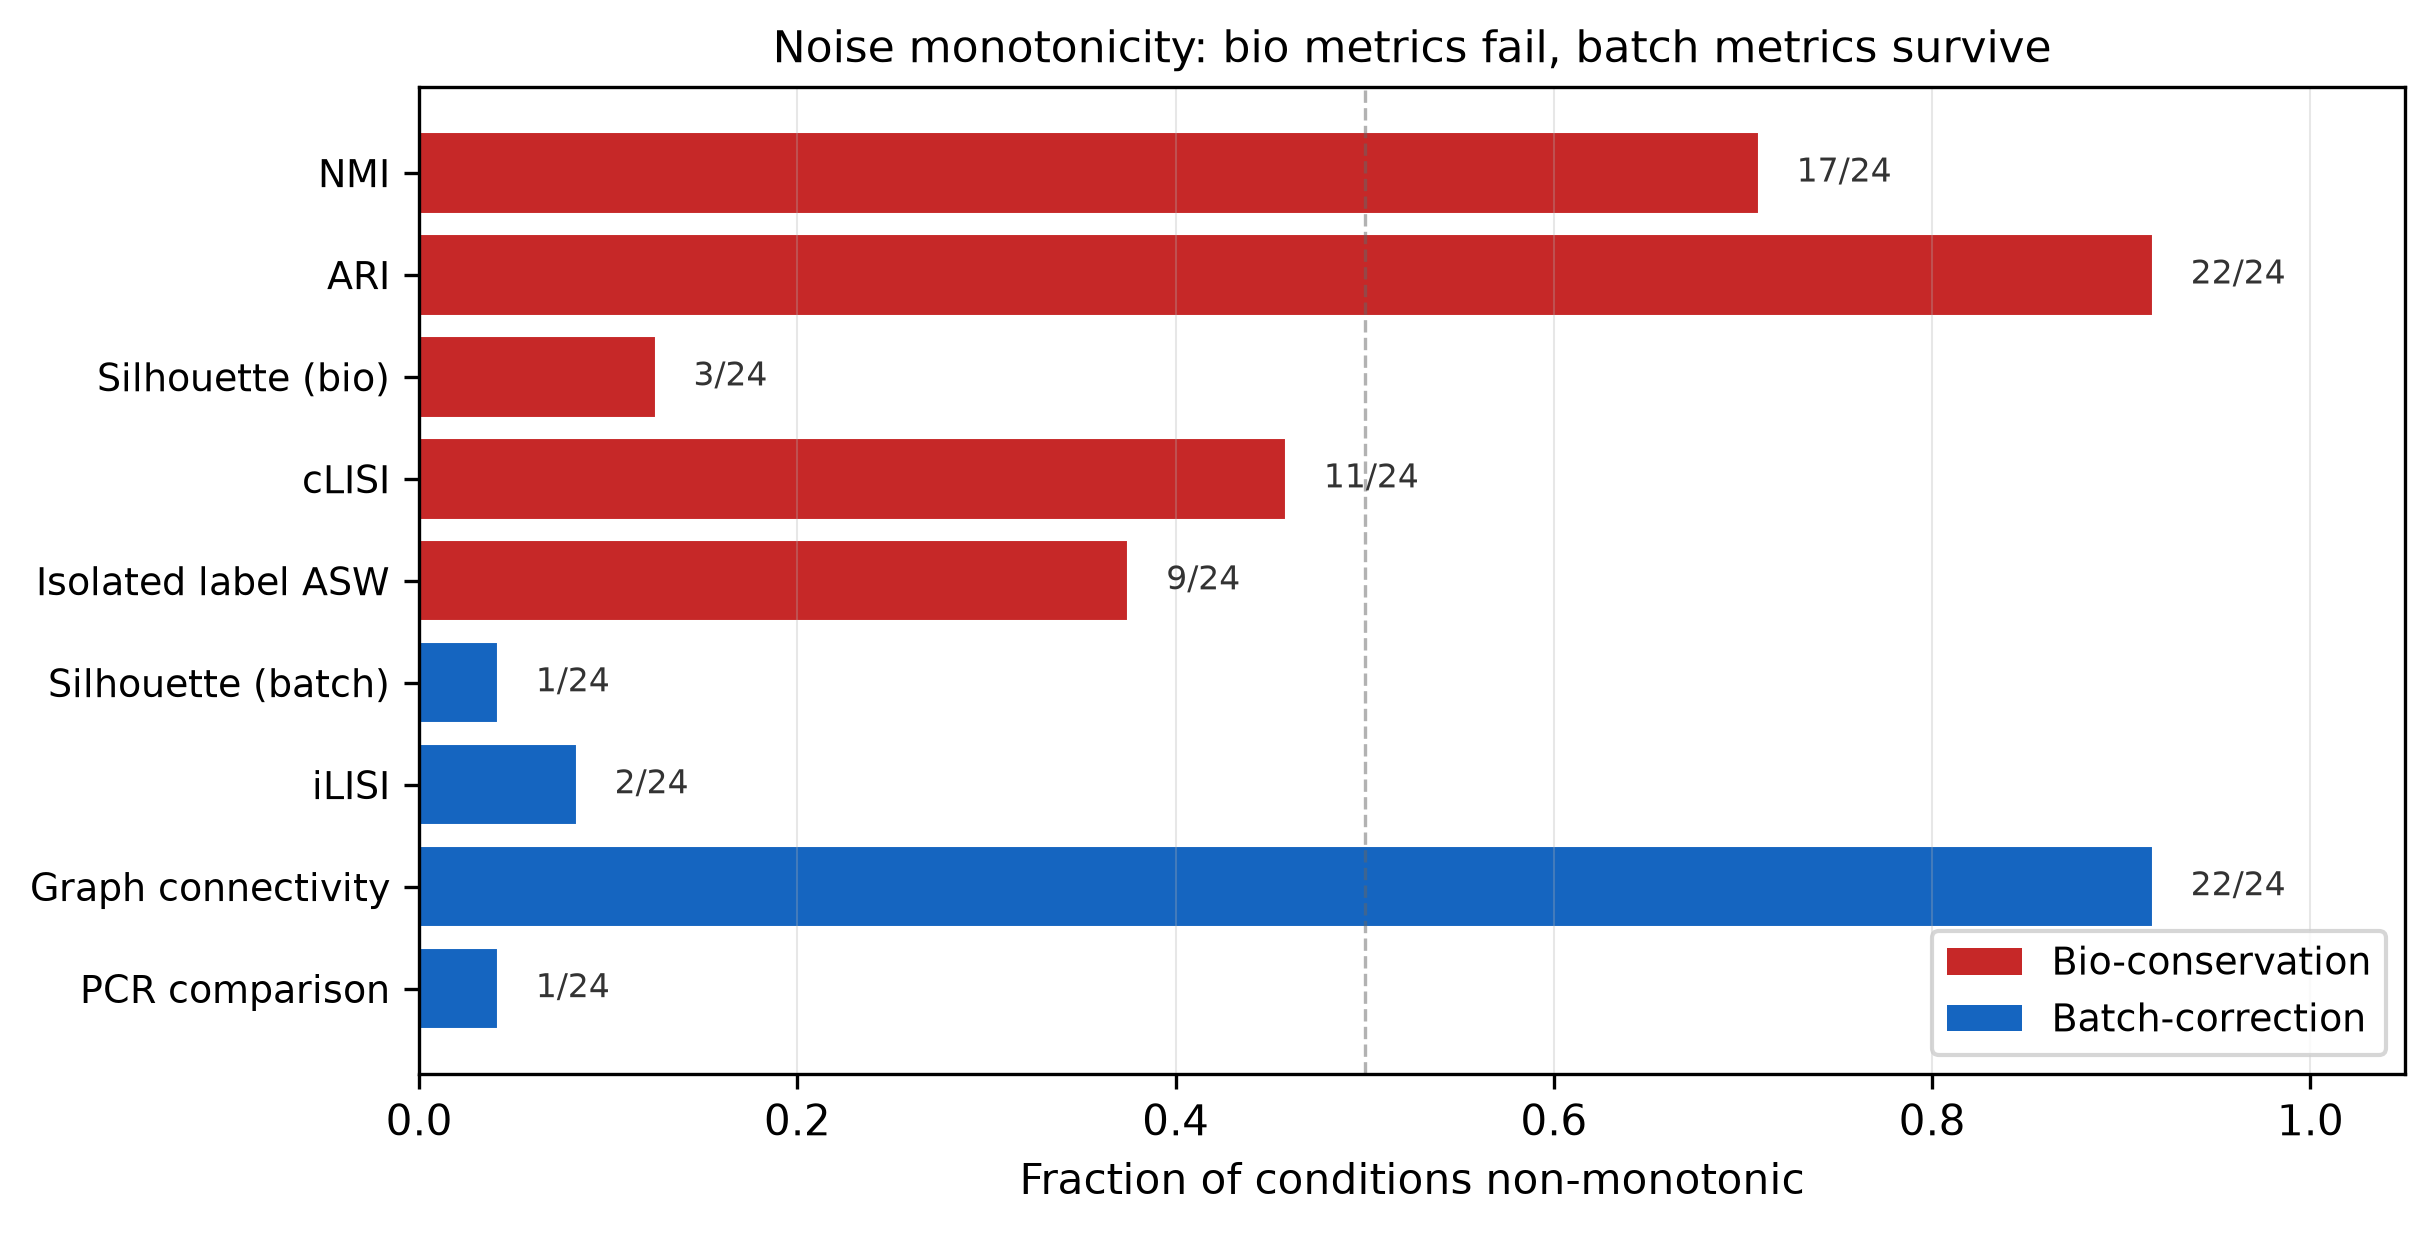
\includegraphics[width=0.75\textwidth]{figures/monotonicity_summary.pdf}
\caption{Non-monotonic fraction per metric (out of 24 conditions). Bio-conservation metrics (red): 3/24 to 22/24. Batch-correction metrics (blue): $\leq$2/24 except graph connectivity (22/24). kBET omitted (all null).}
\label{fig:monotonicity}
\end{figure}

\begin{figure}[htb]
\centering
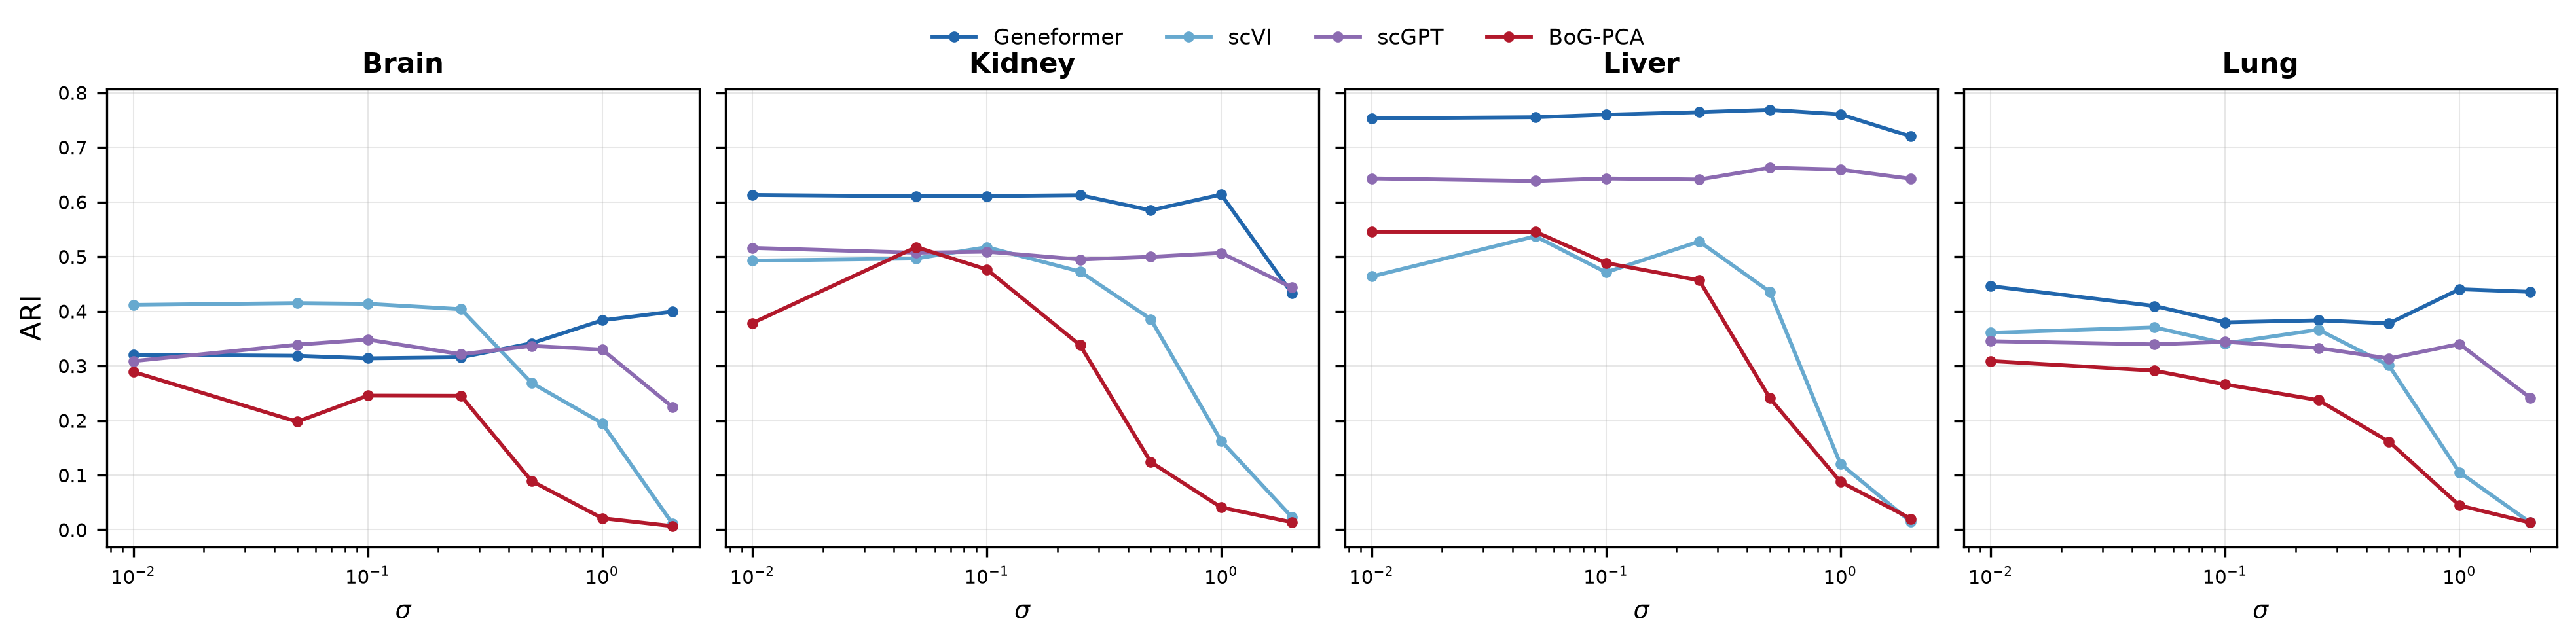
\includegraphics[width=\textwidth]{figures/noise_all_tissues.pdf}
\caption{ARI dose-response across all four tissues. Non-monotonicity is universal: every tissue shows at least one embedding with an initial plateau or increase before collapse. Geneformer is most robust; BoG-PCA collapses fastest.}
\label{fig:noise_tissues}
\end{figure}

\bibliographystyle{plainnat}
\bibliography{paper_d_v11}

\end{document}
